% TASA DE EFICIENCIA EN FUNCIÓN DE LA CANTIDAD DE COMPONENTES PRINCIPALES TOMADAS
\subsection{Test de tasa de eficiencia en función de la cantidad de componentes principales consideradas}
\begin{figure}[H]{}
\centering
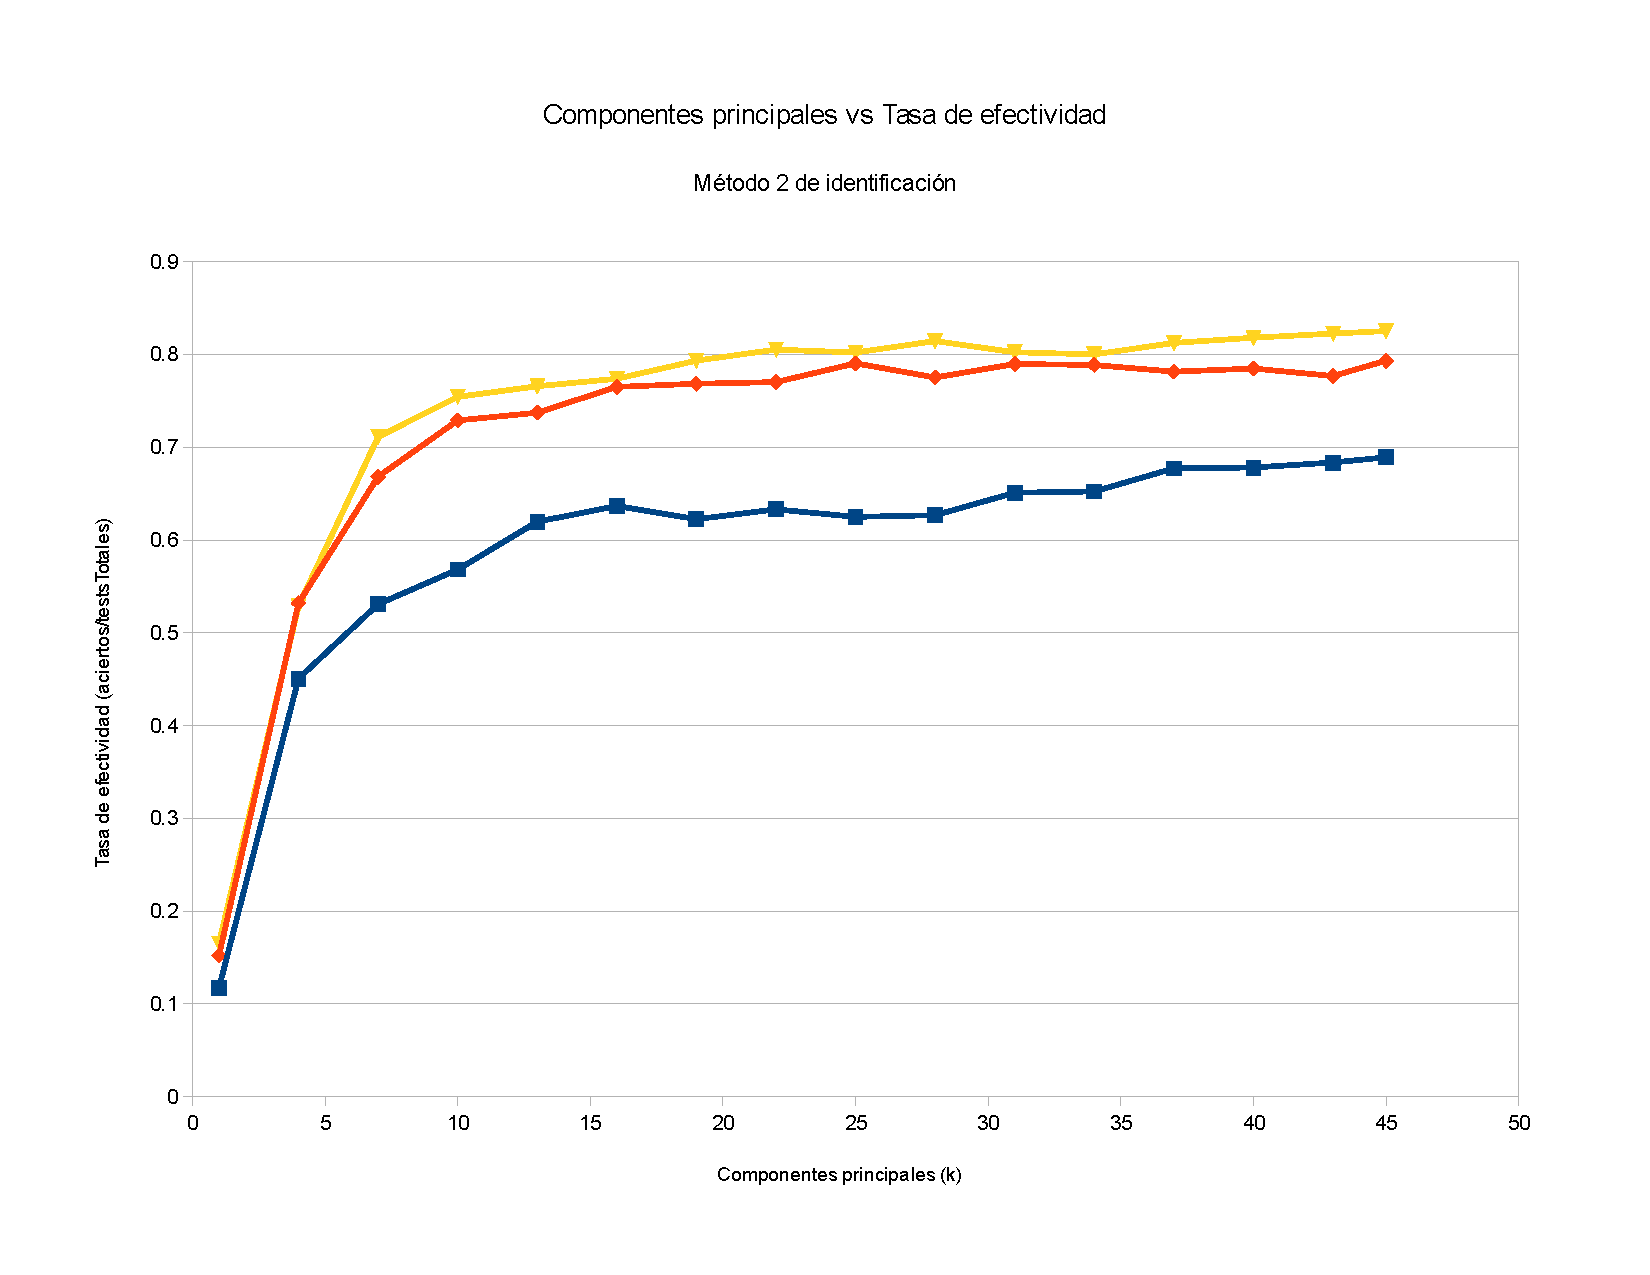
\includegraphics[scale=0.5]{graphs/componentesPrincipalesVsTasaDeEfectividadM2.pdf}
\caption{El método 2 de identificación se corresponde con el de Distancia Mínima Promedio}
\label{CPvsTE}
\end{figure}